
\documentclass[aps,floatfix,prd,showpacs]{revtex4}
%\documentclass[aps,floatfix,prd,showpacs,twocolumn]{revtex4}
\usepackage{graphicx}% Include figure files
\usepackage{dcolumn}% Align table columns on decimal point
\usepackage{bm}% bold math
\usepackage{amsmath}

\voffset 1.0cm

\newcommand{\diff}{\mathrm{d}}
\newcommand{\rhox}{\rho_\chi}
\newcommand{\vesc}{v_{\text{e}}}
\newcommand{\vp}{v^\prime}
\newcommand{\mpr}{m^\prime}
\newcommand{\xp}{x^\prime}
\newcommand{\SA}{S_{\text{A}}}
\newcommand{\SB}{S_{\text{B}}}
\newcommand{\SC}{S_{\text{C}}}
\newcommand{\G}{\text{G}}
\newcommand{\mx}{m_\chi}
\newcommand{\rx}{r_\chi}
\newcommand{\Nx}{N_\chi}
\newcommand{\MDM}{M_{\mathrm{DM}}}
\newcommand{\Rvir}{R_{\mathrm{vir}}}
\newcommand{\Msun}{\textrm{M}_\odot}
\newcommand{\kpc}{\textrm{kpc}}
\newcommand{\gev}{\textrm{GeV}}

\begin{document}


\title{On the Ejection of Dark Matter from Globular Clusters}
\author{T. Hurst and A. Zentner}
\affiliation{
Department of Physics and Astronomy,
University of Pittsburgh,
Pittsburgh, PA 15260,
USA.}

\date{\today}

\begin{abstract}
An abstract is a great convenience for the reader and is required by all journals.
\end{abstract}
\pacs{PACS numbers go here. These are classification codes for your  research. See {\tt http://publish.aps.org/PACS/} for more info.}
\maketitle

%%%%%%%%%%%%%%%%%%%%%%%%%%%%%%%%%%%%%%%%%%%%%%%%%%%
\section{Introduction}
\label{section:intro}

%Modern cosmology is largely centered around the $\Lambda$CDM paradigm.  In this model Dark Matter (DM) composes $\approx 23\%$ of the matter-energy content of the Universe while the remainder is dominated by Dark Energy---parametrized by Einstein's cosmological constant $\Lambda$ \cite{WMAP9,Planck15}. The most compelling particle candidates for the DM are Weakly Interacting Massive Particles (WIMPs).   WIMPs are compelling candidates in part because they can be produced thermally in the early Universe such that they have the correct relic abundance today.  That this happens generically for a particle with a weak-scale cross-section is the so-called `WIMP miracle'.  Moreover, WIMPs arise naturally in extensions to the Standard Model of particle physics and are not merely an ad hoc solution invoked by cosmologists.


%In the $\Lambda$CDM paradigm, DM is the first matter component to collapse and form structures (roughly spherical structures referred to as DM `halos') forming the seeds for all other structure formation {\bf citation needed}.  Baryons collapse within DM halos forming progressively larger and larger structures through the mergers of smaller DM halos.  Thus clusters of galaxies are assembled from galaxies which previously collapsed.  This is referred to as `hierarchical structure formation' and will be the case so long as the DM is `Cold' (non-relativistic at freeze out), hence the C in $\Lambda$CDM.


In the $\Lambda$CDM paradigm, Dark Matter (DM) is the first matter constituent to collapse forming DM halos which serve as the seeds for galaxy formation.  Progressively larger structures are built through the mergers of halos.  This hierarchical structure formation is predicted by theory and is seen in N-body simulations as well as observed in the structure of galaxies and galaxy clusters.  

%One seeming exception to this scenario are Globular Clusters (GC), observations of which indicate that these are not DM dominated objects. Dynamical observations of several GGCs indicate that $M_{\mathrm{DM}} \lesssim M_*$ \cite{Shin,Conroy} where  $M_{\mathrm{DM}}$ is the DM mass and $M_*$ is the stellar mass.  Moreover, observations of the cooling of white dwarfs in GCs indicate that if the DM is indeed a WIMP, then for a large portion of parameter space, the DM content of GCs is likely to be at least 2-3 orders of magnitude less than the stellar content {\bf cite myself and a couple of other references}.  

One seeming exception to this scenario are Globular Clusters (GC).  Ref.~\cite{Peebles1984} was the first to propose that GCs form in extended DM halos.  However, observations of many GCs reveal thin tidal tails which N-body simulations predict should not form if they possess halos.  Moreover recent studies of several GCs indicate that the ratio of the mass in DM to stars in several GCs $\MDM/M_* \lesssim 1$ \cite{Grillmair1995,Odenkirchen2003,Moore1996,Shin, Conroy} and is potentially $\lesssim 10^{-2}$ if the DM is a low mass ($\mx \sim 10\, \gev$) weakly interacting particle \cite{Hurst}.  Though they seemingly do not possess DM halos today, they could have had them in the past and subsequently lost their DM.  One mechanism invoked for the removal of the halo is tridal stripping by the galaxy \cite{Bromm2002,Mashchenko2005}.  While, the majority of the GGCs orbit within strong tidal fields there does exist a population of isolated GCs with galactocentric distances $r_{gc} > 70\, \kpc$ that should not have lost their halos tidally.  Two such GCs are NGC 2419 ($r_{gc} = 89.9\, \kpc$) and MGC1, which at $\sim 200\, \kpc$ from M31 is the most isolated cluster in the local group \cite {Harris, Conroy}.  Obseravtions of both these cluster indicate that $\MDM/M_* \lesssim 1$ \cite{Conroy}.


%Because they are not dominated by DM today, it is generally thought that GCs did not form inside DM halos {\bf citation needed}.  The most likely alternative then is that their formation was triggered by gravitational instability {\bf citation needed}.  However, the formation scenarios of GCs remain controversial in part because of the complex abundance patterns measured in stars.  These observations indicate that GCs must have been much more massive in the past in order to retain significant amounts of heavy elements that would have been ejected by Supernovae \cite{Gratton,Gratton2012,Con&Sperg}.

It is now generally thought GCs formed in gas compressed by shocks \cite{Gunn1980,Harris1994}.  However, the formation scenarios of GCs remain controversial in part because of the complex abundance patterns measured in stars.  These observations indicate that GCs must have been much more massive in the past in order to retain significant amounts of heavy elements that would have been ejected by supernovae \cite{Gratton,Gratton2012,Con&Sperg}.


%One feasible scenario in which GCs could have had more mass in the past is if they formed in DM halos, but then subsequently ejected their DM content through multi-body gravitational interactions.  It is well known that early in their history GCs ejected stars by just this mechanism until the cluster became `relaxed' \cite{HenonA,HenonB}, so it is certainly reasonable to wonder if GCs could have ejected significant amounts of DM in the same manner.


In this paper we investigate an additional mechanism by which GCs could eject DM halos:  through multi-body gravitational effects.  

%In this paper we will investigate the escape rate of DM particles from a spherically symmetric stellar system in order to ascertain just how reasonable the DM ejection scenario is.  As the interaction is gravitiational, we shall not trouble ourselves with the details of the DM particle.  The only assumption we make of the DM particle is that its mass is significantly less than the mass of a typical star, which will be the case in any reasonable physical model.  


%The remainder of the paper is organized as follows:  in \S\ref{section:methods} we present the details of the calculation of the escape rate of DM particles from an isolated, spherical stellar system.  In \S\ref{section:results} we present our results and in \S\ref{section:conclusions} we discuss our conclusions.


%%%%%%%%%%%%%%%%%%%%%%%%%%%%%%%%%%%%%%%%%%%%%%%%%%%
\section{Methods}
\label{section:methods}


Our calculation will follow the approach of a pair of classic papers by H\'{e}non (Refs~\cite{HenonA,HenonB} henceforth Papers 1 \& 2 respectively).  As in Paper 2, we begin with the assumption that the DM and stellar distributions are spherically symmetric and that the particle velocities are isotropic.  Then, the number of DM particles in a volume element $\diff^3r\diff^3v$ is:
%
%  DM particles per volume element
\begin{equation}
(4\pi)^2r^2v^2f(r,v)\diff r\diff v,
\end{equation}
%
%
where $f(r,v)$ is the DM distribution function.  Similarly, if the stellar distribution function is $g(r,\vp,\mpr$) then the number of stars in the volume element $\diff^3r\diff^3\vp \diff \mpr$ is:
%
%  Stars per volume element
\begin{equation}
(4\pi)^2r^2{\vp}^2g(r,\vp,\mpr)\diff r\diff \vp \diff \mpr.
\end{equation}
%
%

Consider a DM particle of mass $\mx$ and coordinates $(r,v)$.  According to Paper 1 the probability that a particle will experience an encounter that takes it from a velocity $\vec{v} \rightarrow \vec{v} + \vec{e}$ is:
%
%  Probability of encounter
\begin{equation}
P = 8\pi \G^2\diff t\frac{\diff^3e}{e^5}\int^\infty_0 {\mpr}^2\,\diff \mpr\int^\infty_{\vp_0}g(r,\vp,\mpr)\vp\,\diff \vp, 
\end{equation}
%
%
where $\vp_0 = \frac{1}{e}|\vec{v}\cdot\vec{e} + \frac{\mx+\mpr}{2\mpr}e^2|$ and G is Newton's constant.  As stated in \S\ref{section:intro}, the one assumption of the DM particle we make is that $\mx \ll \mpr$ so 
%
% \vp_0 with small DM mass
\begin{equation}
\label{v0p1}
\begin{split}
\vp_0 &= \frac{1}{e}|\vec{v}\cdot\vec{e} + \frac{e^2}{2}| \\
&= |v\cos\delta + \frac{e}{2}|.
\end{split}
\end{equation}
%
%
The particle will escape if 
%
% Condition for escape
\begin{equation}
|\vec{v}+\vec{e}| \ge \vesc(r),
\label{geve}
\end{equation}
%
%
where $\vesc(r)$ is the local escape velocity.  In the remainder of the paper we will denote the local escape velocity simply as $\vesc$.  Using the notation of Paper 2, let $e, \delta, \varphi$ be a set of spherical coordinates for the kick velocity $\vec{e}$.  Then from (\ref{geve}) we have that,
%
% 
\begin{equation}
\label{geve2}
v^2 + e^2 + 2ve\cos\delta \ge \vesc^2.
\end{equation}
Then, assuming that the kick velocity distribution is isotropic, we can write the probability that the DM particle will esacpe in a time d$t$ as:
%
% Probability of escape
\begin{equation}
Q = 8\pi\G^2\diff t\int^\infty_0 {\mpr}^2\,\diff \mpr\int^\infty_{\vp_0}g(r,\vp,\mpr)\vp\,\diff \vp\int^{2\pi}_0{}\,\diff \varphi\int{\sin\delta}\,\diff \delta\int{e^{-3}}\,\diff e.
\end{equation}
%
%
For a bound DM particle it must be the case that $v < \vesc$, then from (\ref{geve2})
%
%  Dropping the absolute value from v0p1
\begin{equation}
\vesc^2 \le v^2 + e^2 + 2ve\cos\delta \le \vesc^2 + e^2 + 2ve\cos\delta,
\end{equation}
%
%
therefore,
%
% Dropping the absolute value from v0p1
\begin{equation}
v\cos\delta \ge \frac{-e}{2}.
\end{equation}
%
%
Hence, we can drop the absolute value in (\ref{v0p1}).  Now,
%
%  Probability of escape
\begin{equation}
Q = 16\pi^2\G^2\diff t\int^\infty_0{\mpr}^2\,\diff \mpr\int^\infty_{\vp_0}{g(r,\vp,\mpr)\vp}\,\diff \vp\int{e^{-3}}\,\diff e\int{}\,\diff \cos\delta,
\end{equation}
%
%
where integration should satisfy:
%
% Integration limits
\begin{equation}
-1 \le \cos\delta \le 1
\label{lim1}
\end{equation}
\begin{equation}
0 \le e
\label{lim2}
\end{equation}
\begin{equation}
v^2 + e^2 + 2ve\cos\delta \ge \vesc^2
\label{lim3}
\end{equation}
\begin{equation}
v\cos\delta + \frac{e}{2} \le \vp < \vesc.
\label{lim4}
\end{equation}
%
%
To find the escape rate, we now integrate over the position and veolocity of the DM particle.  Let $\Nx$ be the number of DM particles in the cluster,  
%
%  Definition of Nx
\begin{equation}
\Nx = \int^\infty_0{4\pi r^2}\,\diff r\int^{\vesc}_0{4\pi v^2f(r,v)}\,\diff v\int^\infty_0{\Nx(m)}\,\diff m,
\label{Nchi}
\end{equation}
with $f(r,v)$ normalized to 1 and $\Nx(m) = \Nx\delta(m-\mx)$ assuming the halo is composed of a single DM constituent.  Then the specfic escape rate is:
%
%  Escape rate.  Label esc1
\begin{equation}
\label{esc1}
\begin{split}
\bigg|\frac{1}{\Nx}\frac{\partial \Nx}{\partial t}\bigg| & = \int^\infty_0{4\pi r^2}\,\diff r\int^{\vesc}_0{4\pi v^2\frac{Q}{\diff t}f(r,v)}\,\diff v \\
& = 256\pi^4\G^2\int^\infty_0{r^2}\,\diff r\int^{\vesc}_0{v^2f(r,v)}\,\diff v\int^\infty_0{\mpr}^2\,\diff \mpr\int^\infty_{\vp_0}{g(r,\vp,\mpr)\vp}\,\diff \vp\int{e^{-3}}\,\diff e\int{}\,\diff\cos\delta,
\end{split}
\end{equation}
%
%
with the limits in Eqs. (\ref{lim1}-\ref{lim4}) satisfied and where we have taken the magnitude since $\frac{\partial \Nx}{\partial t}$ is negative.  If the magnitude of the specific escape rate is greater than $\tau^{-1}$ with $\tau$ the age of the Universe, then it is a reasonable proposition that the GC could have ejected its DM halo by the present time.  We normalized Eq.~(\ref{Nchi}) to $\Nx$ rather than 1 to make this point explicit.  

As noted in Paper 2, this expression looks quite intractable, but the integrals in $e$ and $\delta$ can in fact be calculated analytically.  Keeping with the notation of Paper 2 let
% Definition of S
\begin{equation}
S = \int{e^{-3}}\,\diff e\int{}\,\diff \cos\delta,
\end{equation}
%
and let $C = \cos\delta$. From (\ref{lim3})
% Limits on C
\begin{equation}
C \ge \frac{\vesc^2-v^2-e^2}{2ve} = C_1,
\end{equation}
from (\ref{lim4})
\begin{equation}
C \le \frac{\vp - \frac{e}{2}}{v} = C_2,
\end{equation}
and from (\ref{lim1})
\begin{equation}
C_3 = -1 \le C \le 1 = C_4.
\end{equation}
%
%
In order for $S$ to be non-zero we must have that $C_1 < C_4, C_1 < C_2, C_3 < C_4$, and $C_3 < C_2$. Now $C_3 < C_4$ trivially. $C_1 < C_4$ requires that,
%
%  Determining upper and lower bounds for C integral
\begin{equation}
e > \vesc - v = e_1,
\label{e1}
\end{equation}
which is stronger than (\ref{lim2}). $C_1 < C_2$ requires that,
\begin{equation}
e > \frac{\vesc^2 - v^2}{2\vp} = e_2,
\label{e2}
\end{equation}
which is again stronger than (\ref{lim2}).  And $C_3 < C_2$ requires that,
\begin{equation}
e < 2(\vp + v) = e_3,
\label{e3}
\end{equation}
which further restricts (\ref{lim2}).  $C_3$ will be the lower limit of the $\diff C$ integral when $C_1 < C_3$ or when 
\begin{equation}
e > v + \vesc = e_4,
\end{equation}
and $C_2$ will be the upper limit when $C_2 < C_4$ or when 
\begin{equation}
e > 2(\vp - v) = e_5.  
\end{equation}
%
%
Thus, in order to determine the limits of the integrals in $S$, we must consider the order of $e_1, e_2, e_3, e_4$, and $e_5$.  Elementary calculations show that 
% 
% order of the e_i
\begin{equation}
\begin{split}
	\vp \ge \frac{1}{2}(\vesc - 3v) = \vp_1 &\Rightarrow e_1 \le e_3\\
	\vp \ge \frac{1}{2}(\vesc - v) = \vp_2 &\Rightarrow e_2 \le e_3, e_2 \le e_4, e_4 \le e_3\\
	\vp \ge \frac{1}{2}(\vesc + v) = \vp_3 &\Rightarrow e_2 \le e_1, e_1 \le e_5, e_2 \le e_5\\
	\vp \ge \frac{1}{2}(\vesc + 3v) = \vp_4 &\Rightarrow e_4 \le e_5\\
\end{split}
\end{equation}
%
%
and it is always true that $e_1 \le e_4$ and $e_5 \le e_3$.  These relations divide the $v$-$ \vp$ plane into 5 regions A, B, C, D, and E (see Fig.~\ref{regions}).  In region A,
%
% order in region A
\begin{equation}
e_5 \le e_1 \le e_2 \le e_4 \le e_3. 
\end{equation} 
%
%
Thus in region A we have,
%
% SA
\begin{equation}
\begin{split}
\SA & = \int^{e_4}_{e_2}{e^{-3}}\,\diff e\int^{C_2}_{C_1}\,\diff C + \int^{e_3}_{e_4}{e^{-3}}\,\diff e\int^{C_2}_{C_3}\,\diff C \\
& = \frac{2{\vp}^3}{3v(\vesc^2 - v^2)^2} + \frac{1}{8v(\vp + v)} - \frac{2\vesc + v}{6v(\vesc + v)^2}.
\end{split}
\end{equation}
%
%
In region B,
%
% order in region B
\begin{equation}
e_2 \le e_1 \le e_5 \le e_4 \le e_3.
\end{equation}
%
%
Hence,
%
%  SB
\begin{equation}
\begin{split}
\SB & = \int^{e_5}_{e_1}{e^{-3}}\,\diff e\int^{C_4}_{C_1}\,\diff C + \int^{e_4}_{e_5}{e^{-3}}\,\diff e\int^{C_2}_{C_1}\,\diff C + \int^{e_3}_{e_4}{e^{-3}}\,\diff e\int^{C_2}_{C_3}\,\diff C \\
& = \frac{3\vesc^2 - v^2}{3(\vesc - v)^2(\vesc+v)^2} - \frac{1}{4({\vp}^2 - v^2)}.
\end{split}
\end{equation}
%
%
In region C,
%
%  order in region C
\begin{equation}
e_2 \le e_1 \le e_4 \le e_5 \le e_3.
\end{equation}
%
%
Hence,
%
%  SC
\begin{equation}
\begin{split}
\SC & = \int^{e_4}_{e_1}{e^{-3}}\,\diff e\int^{C_4}_{C_1}\,\diff C + \int^{e_5}_{e_4}{e^{-3}}\,\diff e\int^{C_4}_{C_3}\,\diff C + \int^{e_3}_{e_5}{e^{-3}}\,\diff e\int^{C_2}_{C_3}\,\diff C \\
& = \frac{3\vesc^2 - v^2}{3(\vesc - v)^2(\vesc+v)^2} - \frac{1}{4({\vp}^2 - v^2)}\\
&= \SB.
\end{split}
\end{equation}
%
%
In region D,
%
% order in D
\begin{equation}
e_5 \le e_3 \le e_1 \le e_4 \le e_2.
\end{equation}
%
%
Here we can not simultaneously satisfy $e > e_1, e > e_2,$ and $e < e_3$, thus region D is forbidden.  In region E,
%
% order in E
\begin{equation}
e_5 \le e_1 \le e_3 \le e_4 \le e_2.
\end{equation}
%
%
So region E is forbidden for the same reason as D.  Then Eq. (\ref{esc1}) becomes,
%
%  Escape rate esc2
\begin{equation}
\label{esc2}
\begin{split}
\bigg|\frac{1}{\Nx}\frac{\partial \Nx}{\partial t}\bigg| = 256\pi^4\G^2\int^\infty_0{r^2}\,\diff r\int^\infty_0{\mpr}^2\,\diff \mpr \times&\Bigg\{\int^{\vesc}_0{v^2f(r,v)}\,\diff v\int^{\vp_3}_{\vp_2}{\vp \SA g(r,\vp,\mpr)}\,\diff \vp \\
 &+ \int^{\vesc/3}_0{v^2f(r,v)}\,\diff v\int^{\vp_4}_{\vp_3}{\vp \SB g(r,\vp,\mpr)}\,\diff \vp \\ &+ \int^{\vesc}_{\vesc/3}{v^2f(r,v)}\,\diff v\int^{\vesc}_{\vp_3}{\vp \SB g(r,\vp,\mpr)}\,\diff \vp \\
&+\int^{\vesc/3}_0{v^2f(r,v)}\,\diff v\int^{\vesc}_{\vp_4}{\vp \SB g(r,\vp,\mpr)}\,\diff \vp\Bigg\}.
\end{split}
\end{equation}
%
% Figure of integration limits
\begin{figure}[htp]
\centering
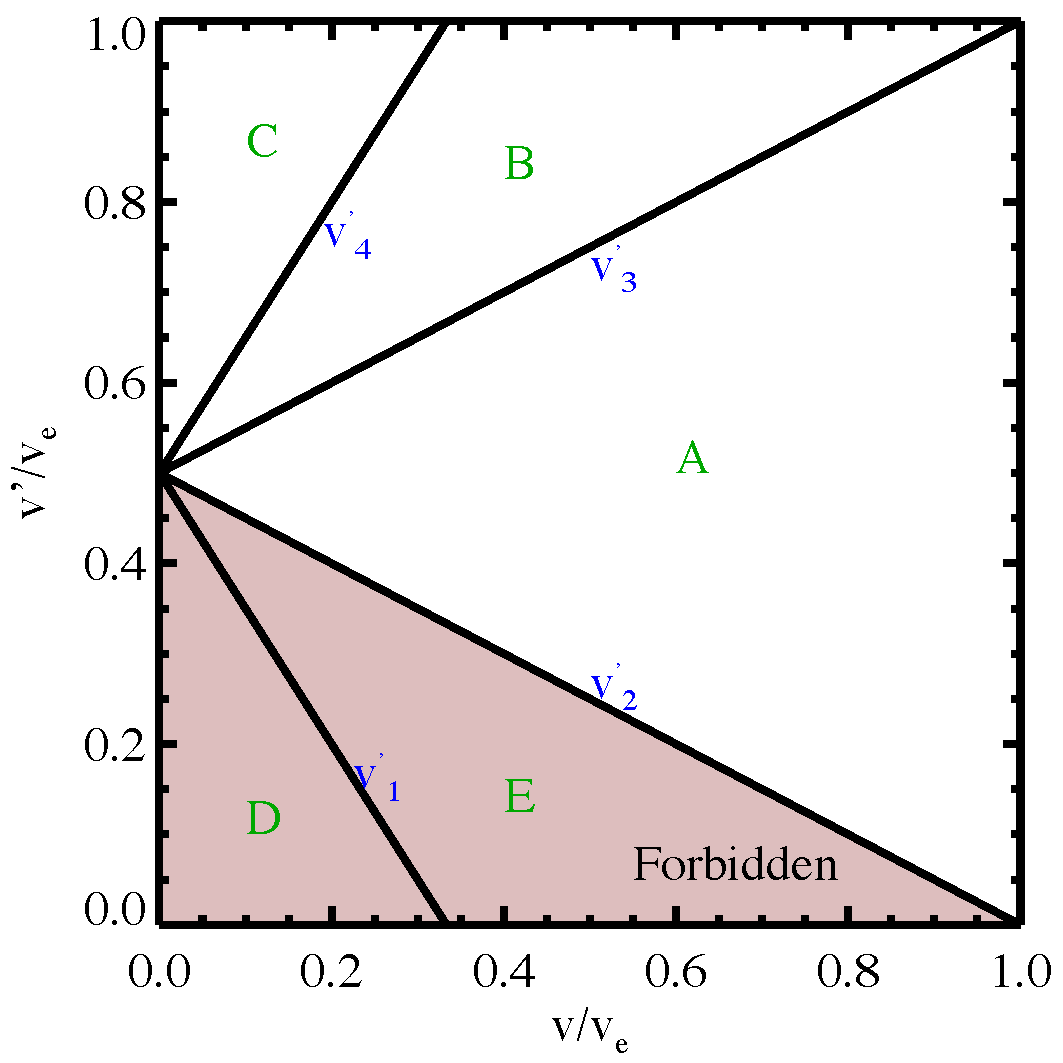
\includegraphics[width=9cm, height=9cm]{regions}
\caption{The integration regions over the kick velocity $\vec{e}$.  The shading denotes the fact that regions D \& E are forbidden because we cannot simultaneously satisfy all of the required inequalities in Eqs.~(\ref{lim1}-\ref{lim4}).}
\label{regions}
\end{figure}
%
%

In order to proceed further we must specify the stellar and DM distribution functions.  As in Paper 2, we take for the stellar component a Plummer model
%
%  The stellar density
\begin{equation}
	\rho_*(r) = \frac{3M_*}{4\pi}\frac{r_0^2}{(r^2+r_0^2)^{5/2}},
%g(r,\vp,\mpr) = \frac{24\sqrt{2}N(\mpr)}{7\pi^3r_0^3\psi_0^5}\bigg(\frac{\vesc^2 - {\vp}^2}{2}\bigg)^\frac{7}{2},
\end{equation}
where $r_0$ is the half-mass radius of the GC.  As there is little guidance on what the distribution function of DM in a GC might be, we will also use a Plummer model for the DM
%
 % The DM density
\begin{equation} 
	\rho_\chi(r) = \frac{3\MDM}{4\pi}\frac{\rx^2}{(r^2+\rx^2)^{5/2}},
%f(r,v) = \frac{24\sqrt{2}}{7\pi^3r_0^3\psi_0^5}\bigg(\frac{\vesc^2 - {v}^2}{2}\bigg)^\frac{7}{2}
\end{equation}
%
%
where $\rx$ is the half-mass radius of the DM halo.  We choose the Plummer model for the DM in part because it has some nice mathematical properties that make it a convenient choice.  As we shall see below, the Plummer distribution function allows us to separate the radial and velocity integrals.  There is also a factor of $\big(\frac{\vesc^2 - {v}^2}{2}\big)^{7/2}$ in the distribution function which cancels out the divergence of ($\vesc^2 - v^2)^{-2}$ in $\SA$.  
%
%

Now the gravitational potential is
%
%  The gravitational potential
\begin{equation} 
	\phi(r) = \frac{-GM_*}{\Big(r^2+r_0^2\Big)^{1/2}} + \frac{-G\MDM}{\Big(r^2+\rx^2\Big)^{1/2}}.
\end{equation}
%
%
In general the half-mass radii of the 2 components need not be the same.  If $\rx \neq r_0$ the analytic expressions needed to derive the distribution function become cumbersome and we treat this case numerically (see Fig.~\ref{dist func}).  In the case that $r_0 = \rx$ we will have the standard Plummer distribution
%
 % The DM distribution function
\begin{equation} 
	f(r,v) = \frac{24\sqrt{2}}{7\pi^3r_0^3\psi_0^5}\bigg(\frac{\vesc^2 - {v}^2}{2}\bigg)^\frac{7}{2}
\end{equation}
%
%
where $\psi_0 = \frac{\G M}{r_0}$ with $M = M_* + M_{\mathrm{DM}}$ the total mass of the cluster and $E = \frac{-3\pi\psi_0^2r_0}{64\G}$ its energy.  
%
% Figure of the distribution function f(r,v)
\begin{figure}[htp]
\centering
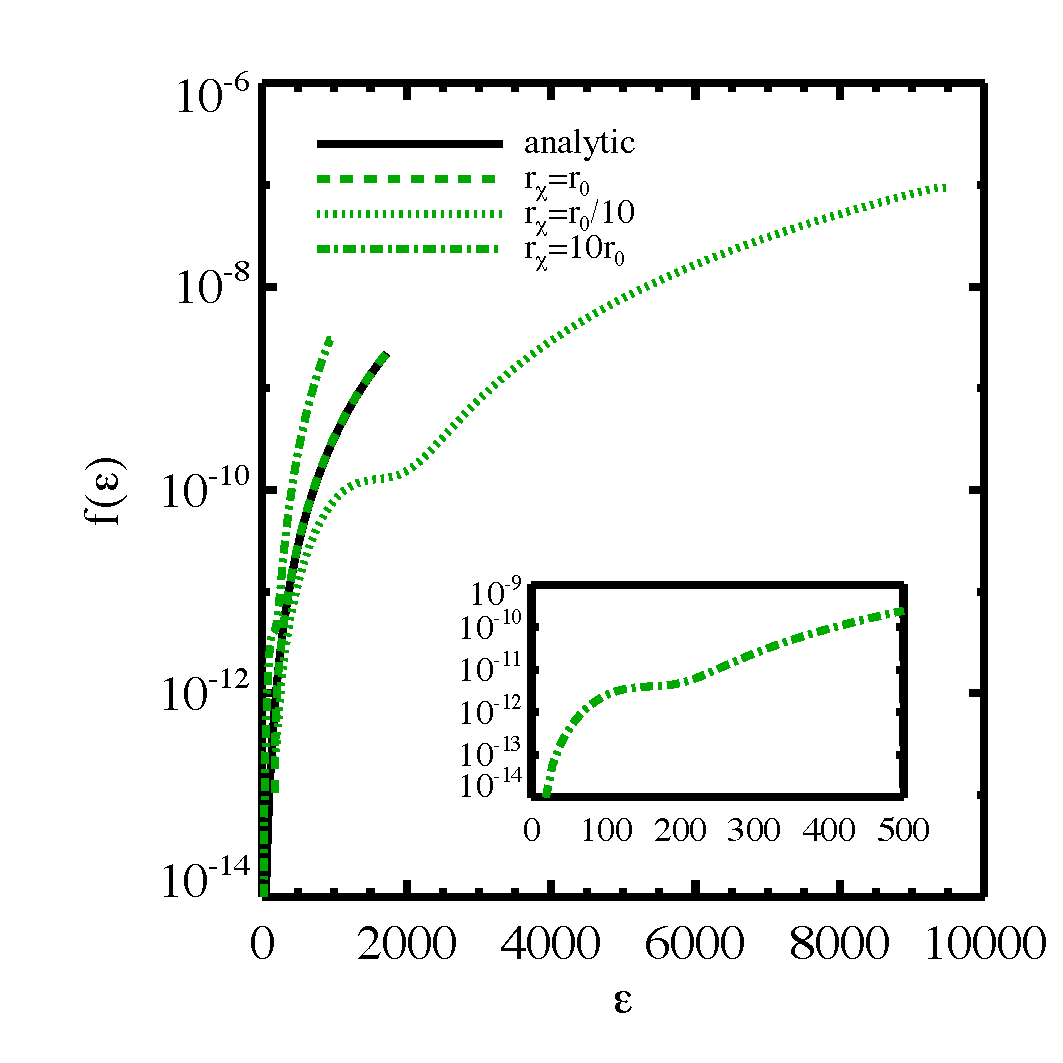
\includegraphics[width=12cm, height=12cm]{Plummer_Compare}
\caption{The distribution function $f(\varepsilon)$ as a function of the magnitude of the specific energy \big($\varepsilon = \frac{1}{2}[\vesc^2-v^2]\big).$}  The solid line is the standard Plummer model in the case that $\rx = r_0$.  The dashed green line shows the numerical result for this case which is in agreement with the analytic case.  The dotted line shows the distribution function in the case that $\rx = r_0/10$ while the dot-dashed line shows the case where $\rx = 10r_0$.  The inset is a zoom in of the latter case, showing the feature at $\varepsilon \approx 150$.
\label{dist func}
\end{figure}
%
%

With the choice that $\rx = r_0$ we have that 
%
%  The escape speed
\begin{equation}
	\begin{split}
	\vesc &= \sqrt{2\psi} \\
		&= \frac{(2\psi_0)^{1/2}}{\big(1+\frac{r^2}{r_0^2}\big)^{1/4}},
	\end{split}
\end{equation}
%
%
where we have defined $\psi(r) = -\phi(r)$.  Defining the stellar mass spectrum $N_*(m)\diff m$ as the number of stars in the mass interval $m \rightarrow m+\diff m$, we have that $g(r,\vp,\mpr) = f(r,\vp)N_*(\mpr)$.  Then Eq.~\ref{esc2} becomes
%
%  Escape rate esc3
\begin{equation}
\label{esc3}
\begin{split}
\bigg|\frac{1}{\Nx}\frac{\partial \Nx}{\partial t}\bigg| = \frac{2304\G^2}{49\pi^2 r_0^6\psi_0^{10}}\int^{\Rvir}_0{r^2}\,\diff r\int^\infty_0{N_*(\mpr)\mpr}^2\,\diff \mpr \times &\Bigg\{ \int^{\vesc}_0{v^2(\vesc^2 - {v}^2)^\frac{7}{2}}\,\diff v\int^{\vp_3}_{\vp_2}{\vp \SA{(\vesc^2-{\vp}^2})^{7/2}}\,\diff \vp \\
&+ \int^{\vesc/3}_0{v^2(\vesc^2 - {v}^2)^\frac{7}{2}}\,\diff v\int^{\vp_4}_{\vp_3}{\vp \SB{(\vesc^2-{\vp}^2})^{7/2}}\,\diff \vp \\ &+ \int^{\vesc}_{\vesc/3}{v^2(\vesc^2 - {v}^2)^\frac{7}{2}}\,\diff v\int^{\vesc}_{\vp_3}{\vp \SB{(\vesc^2-{\vp}^2})^{7/2}}\,\diff \vp \\
&+ \int^{\vesc/3}_0{v^2(\vesc^2 - {v}^2)^\frac{7}{2}}\,\diff v\int^{\vesc}_{\vp_4}{\vp \SB{(\vesc^2-{\vp}^2})^{7/2}}\,\diff \vp\Bigg\}.
\end{split}
\end{equation}
%
%
where the virial radius $\Rvir$ of the DM halo is chosen to be suitably large $(\sim 10r_0)$such that the integrals in Eq.~(\ref{esc3}) are all converged.  


Continuing the approach of Paper 2, we now define new variables: 
%
% definition of x and x'
\begin{equation} 
	x = v/\vesc, \qquad \xp = \vp/\vesc.	
\end{equation}
%
%
Then we can remove $\vesc$ from the integrals over $v$ and $\vp$ and perform those integrals seperately from the radial integral.  It is proven in Appendix II of Paper 2 that the Plummer model is the only steady state distribution for which this separation is possible.  Then Eq.~(\ref{esc3}) becomes
%
% Escape rate esc4
\begin{equation}
\label{esc4}
\begin{split}
\bigg|\frac{1}{\Nx}\frac{\partial \Nx}{\partial t}\bigg| = \frac{2304\G^2}{49 r_0^6\psi_0^{10}}\int^{\Rvir}_0{\vesc^{17}r^2}\,\diff r\int^\infty_0{N_*(\mpr)\mpr}^2\,\diff \mpr \times &\Bigg\{ \int^1_0{x^2(1 - x^2)^\frac{7}{2}}\,\diff x\int^{\xp_3}_{\xp_2}{\xp \SA^\prime{(1-{\xp}^2})^{7/2}}\,\diff \xp \\
&+ \int^{1/3}_0{x^2(1 - x^2)^\frac{7}{2}}\,\diff x\int^{\xp_4}_{\xp_3} {\xp \SB^\prime{(1-{\xp}^2})^{7/2}}\,\diff \xp \\ &+ \int^1_{1/3}{x^2(1 - x^2)^\frac{7}{2}}\,\diff x\int^1_{x_3^\prime}{\xp \SB^\prime{(1-{\xp}^2})^{7/2}}\,\diff \xp \\
&+ \int^{1/3}_0{x^2(1 - {x}^2)^\frac{7}{2}}\,\diff x\int^1_{\xp_4}{\xp \SB^\prime{(1-{\xp}^2})^{7/2}}\,\diff \xp\Bigg\},
\end{split}
\end{equation}
%
%
where
%
% xp integral limits 
\begin{equation}
\begin{split}
	\xp_2 &= \frac{1}{2}(1 - x) \\
	\xp_3 &= \frac{1}{2}(1 + x) \\
	\xp_4 &= \frac{1}{2}(1 + 3x),
\end{split}
\end{equation}
%
%
and the $\prime$ in $S_i^\prime$ denotes the fact that it is now a function of $x$ and $\xp$ with $\vesc$ factored out.

Let us now choose a particular stellar mass spectrum.  We begin with the Initial Mass Function (IMF) from Ref.~\cite{Kroupa2001}.  All of the GGCs should have ages of order $\sim10$ Gyr, meaning that their Main Sequence (MS) turnoffs should be at approximately $1\, \Msun$.  Therefore, in order to obtain a crude approximation of the present day stellar mass spectrum, we simply cut off the IMF at $1\, \Msun$.  Note that this is highly conservative as stellar remnants such as Neutron Stars, White Dwarfs, and Black Holes as well as any stars still on the Giant and Horizontal Branches should contribute to the escape rate.  Furthermore, higher mass stars are given more wait in the integral over mass in Eq.~(\ref{esc4}) (see Fig.~\ref{IMF}).

With this choice of stellar mass spectrum we have that
%
% Integral over mass spectrum
\begin{equation}
	\int^\infty_0{N_*(\mpr)\mpr}^2\,\diff \mpr = 0.18M.
\end{equation}
%
%
%
% Figure of stellar mass spectrum
\begin{figure}[htp]
\centering
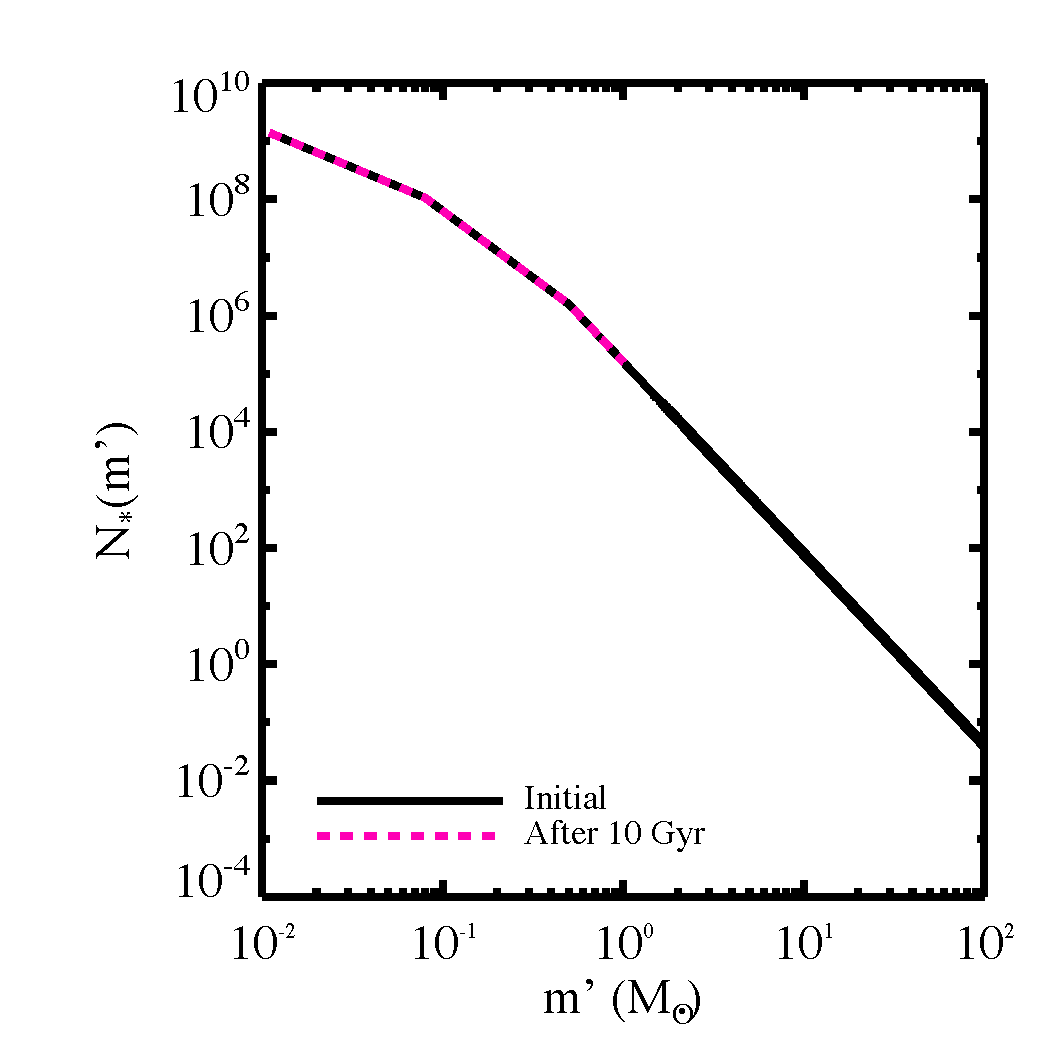
\includegraphics[width=12cm, height=12cm]{IMF}
\caption{The solid black line is the IMF from Ref.~\cite{Kroupa2001}. After 10 Gyr (the approximate age of a GGC) stars more massive than $1\, \Msun$ will have left the MS.  We therefore cut the IMF off at $1\, \Msun$ in order to approximate the present day stellar mass spectrum.  This is a highly conservative choice as the remnants of more massive stars and stars still on the Giant and Horizontal Branches should also contribute to the escape rate.}
\label{IMF}
\end{figure}
%
%

%%%%%%%%%%%%%%%%%%%%%%%%%%%%%%%%%%%%%%%%%%%%%%%%%%%
\section{Results}
\label{section:results}


In Fig.~\ref{EscapePlummer1} we consider the result of integrating Eq.~(\ref{esc4}) numerically for different values of the ratio $\MDM/M_*$ and compare these results to the GGCs (as well as the cluster MGC1 located in M31).  As noted in \S\ref{section:intro}, most of the GGCs could have lost their DM halos through tidal interactions with the Galaxy.  We shall therefore pay particular attention to the most isolated GCs (galactocentric distance $R_{gc} > 70\, \kpc$).  First consider the upper left panel.  For large values of $\MDM/M_*$ the escape rate is much too low for a significant portion of the halo to have been ejected.  However, observations of several GCs (NGC 6397, MGC1, NGC2419) indicate that $\MDM/M_* \lesssim 1$ \cite{Shin,Conroy}.  While NGC 6397 could have had its halo tidally stripped, MGC1 and NGC 2419 are extremely isolated (at 200 kpc away from M31, MGC1 is the most isolated cluster in the local group while NGC 2419 lies some 90 kpc from the center of the MW) and therefore orbit in weak tidal fields and should have retained their primordial DM halos \cite{Conroy}.  Our results therefore rule out the possibility that these clusters formed with significant DM halos.  The remaining panels demonstrate that regardless of the value of $\MDM/M_*$ GCs cannot have ejected a significant amount of DM by multi-body interactions.  Note that the escape rate is no longer sensitive to the value of $\MDM/M_*$ once this ratio has dropped below $\approx 10^{-2}$.
%
% Figure of Specific escape rate all clusters
\begin{figure}[htp]
\centering
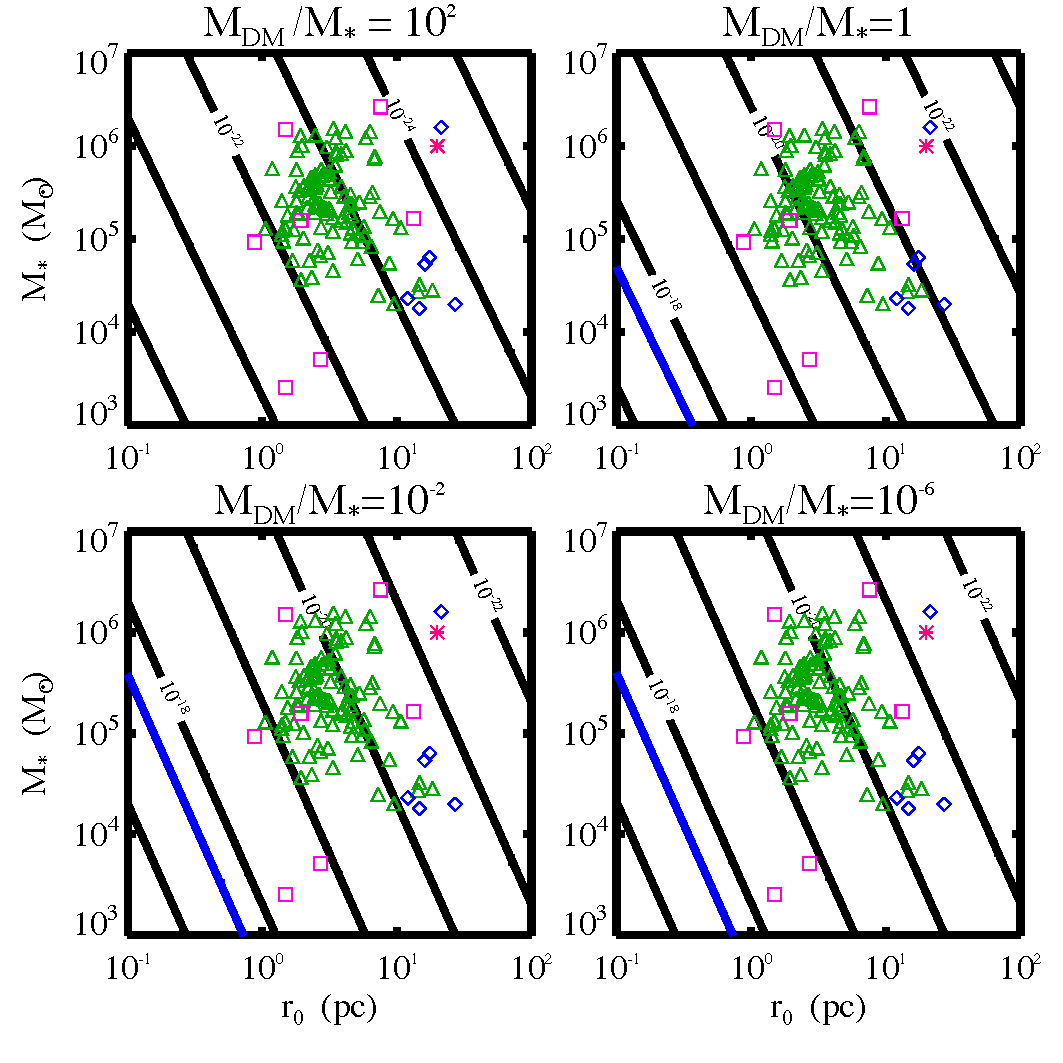
\includegraphics[width=12cm, height=12cm]{EscapePlummer}
\caption{Contours of the specific escape rate for GCs with $r_0 = \rx$.  Each panel shows a different value of the ratio $\MDM/M_*$.  The red star represents MGC1, an isolated cluster orbiting M31, while the blue diamonds represent the isolated popluation of GGCs ($R_{gc} > 70$ kpc).  These isolated GCs are further considered in Fig.~\ref{var_rad_iso}.  GGCs that have been selected for further investigation in Fig.~\ref{var_rad_not_iso} are marked with pink squares while the green triangles denote the remaining GGCs.  The solid blue line is the location where the specific escape rate is $1/\tau$ with $\tau = 13.8$ Gyr the approximate age of the Universe \cite{WMAP9,Planck15}.  GCs with escape rates comparable to or exceeding this limit should have ejected a significant portion of their DM halos.  However, none of the clusters reach this limit regardless of the value of $\MDM/M_*$, with the most massive halos having the lowest escape rates as expected.}  
\label{EscapePlummer1}
\end{figure}

In Figs.~\ref{var_rad_not_iso}~\&~\ref{var_rad_iso} we consider the effect of varying $\rx$ with respect to $r_0$ with $\MDM/M_* = 1$.  We consider $\rx = 10r_0$ which might correspond to an extended primordial halo as well as $\rx = 10^{-1}r_0$ which might correspond to a cluster which has had the outer part of its DM halo stripped by tidal interactions.  The results are obtained by integrating Eq.~(\ref{esc2}) with the appropriate numerically derived distribution functions (see Fig.~\ref{dist func}).  We first consider the GCs marked with pink squares in Fig.~\ref{EscapePlummer1}.  The parameters for these clusters are summarized in Table~\ref{table_not_iso} and span the full range of GGCs.  Note that decreasing (increasing) $\rx$ increases (decreases) the escape rate.  This result is perhaps counter intuitive as a smaller (larger) halo should have a deeper (shallower) potential well which is correspondingly more (less) difficult to escape from.  However, in a smaller (larger) halo, the probability of experiencing an encounter is much higher (lower), which explains the results.  Note, that for $\MDM/M_* = 1$ the only halo which exceeds $1/\tau$ is that of Pal 1 in the case that $\rx = 10^{-1}r_0$.  However, the escape rate can be increased by an additional order of magnitude for smaller values of the ratio $\MDM/M_*$.  Fig~\ref{var_rad_not_iso} then indicates that clusters with $\MDM/M_*~\lesssim~10^{-2}$ and $r_0$~not more than a few parsecs, could have ejected a small remnant halo after the initial halo was tidally stripped.  
%
% Figure of selected GCs not iso
\begin{figure}[htp]
\centering
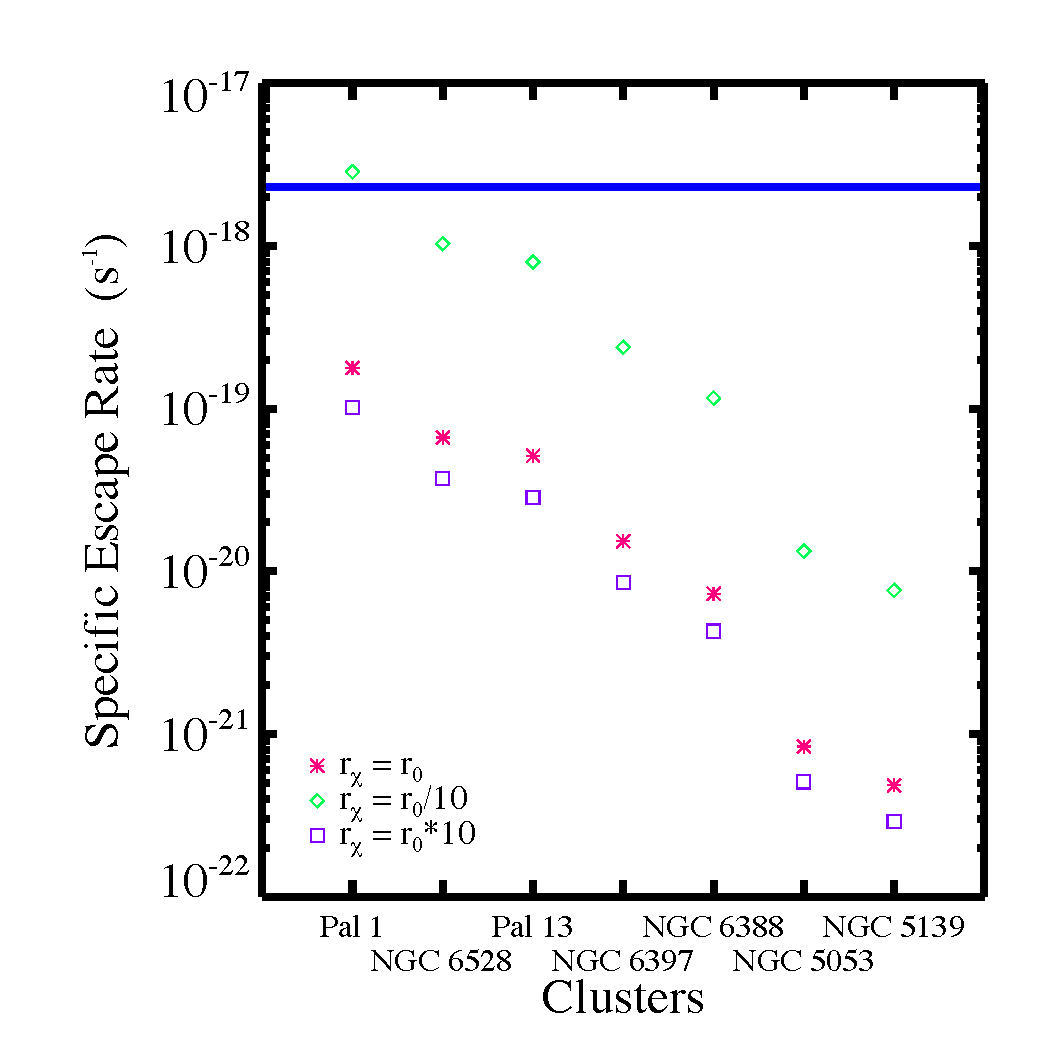
\includegraphics[width=12cm, height=12cm]{var_rad_not_iso}
\caption{Escape rates for several GGCs for different values of $\rx/r_0$ under the assumption that $\MDM/M_* = 1$.  The solid blue line denotes $1/\tau$.}  
\label{var_rad_not_iso}
\end{figure}
%
%
%
%  Table of GC parameters
\begin{table}
\begin{tabular}{ | c | c | c | c |}
	\hline
	GC & $M_* (\mathrm{M}_\odot)$ & $r_0$ (pc) & $\MDM/M_*$ \\
	\hline
  	Pal 1 & $2.54\times10^3$ & 1.49 & ---\\
  	Pal 13 & $5.12\times10^3$ & 2.72 & ---\\
	NGC 5053 & $1.66\times10^5$ & 13.2 & ---\\
	NGC 5139 & $2.64\times10^6$ & 7.56 & ---\\
	NGC 6388 & $1.50\times10^6$ & 1.50& ---\\
	NGC 6397 & $1.59\times10^5$ & 1.94 & $\lesssim 1$\ \cite{Shin}\\
	NGC 6528 & $9.31\times10^4$ & 0.87 & ---\\
	\hline
\end{tabular}
\caption{Parameters for the GCs marked with pink squares in Fig.~\ref{EscapePlummer1} and selected for further consideration in Fig.~\ref{var_rad_not_iso} \cite{Harris}.}
\label{table_not_iso}
\end{table}

In Fig.~\ref{var_rad_iso} we consider the escape rates for the most isolated clusters in the Milky Way (and M31) which are marked with blue diamonds in Fig~\ref{EscapePlummer1}.  The parameters for these clusters are summarized in Table~\ref{table_iso}
%
% Table of isolated GC parameters
\begin{table}
\begin{tabular}{ | c | c | c | c | c |}
	\hline
	GC & $M_* (\mathrm{M}_\odot)$ & $r_0$ (pc) & $R_{gc}$ (kpc) & $\MDM/M_*$\\
	\hline
  	AM 1 & $1.81\times10^4$ & 14.7 & 124.6 & ---\\
  	Eridanus & $2.30\times10^4$ & 12.1 & 95.0 & ---\\
	Pal 3 & $6.38\times10^4$ & 17.5 & 95.7 &---\\
	Pal 4 & $5.41\times10^4$ & 16.1 & 111.2 & ---\\
	NGC 2419 & $1.60\times10^6$ & 21.4& 89.9 &$\lesssim 1$\ \cite{Conroy} \\
	Pal 14 & $2.00\times10^4$ & 27.1 & 71.6 & --- \\
	MGC 1 & $1\times10^6$ & 20 & 200 & $\lesssim 1$\ \cite{Conroy}  \\
	\hline
\end{tabular}
\caption{Parameters for the isolated GCs marked with blue diamonds in Fig.~\ref{EscapePlummer1} and selected for further consideration in Fig.~\ref{var_rad_iso} \cite{Harris}.}
\label{table_iso}
\end{table}
%
% Figure of selected GCs iso
\begin{figure}[htp]
\centering
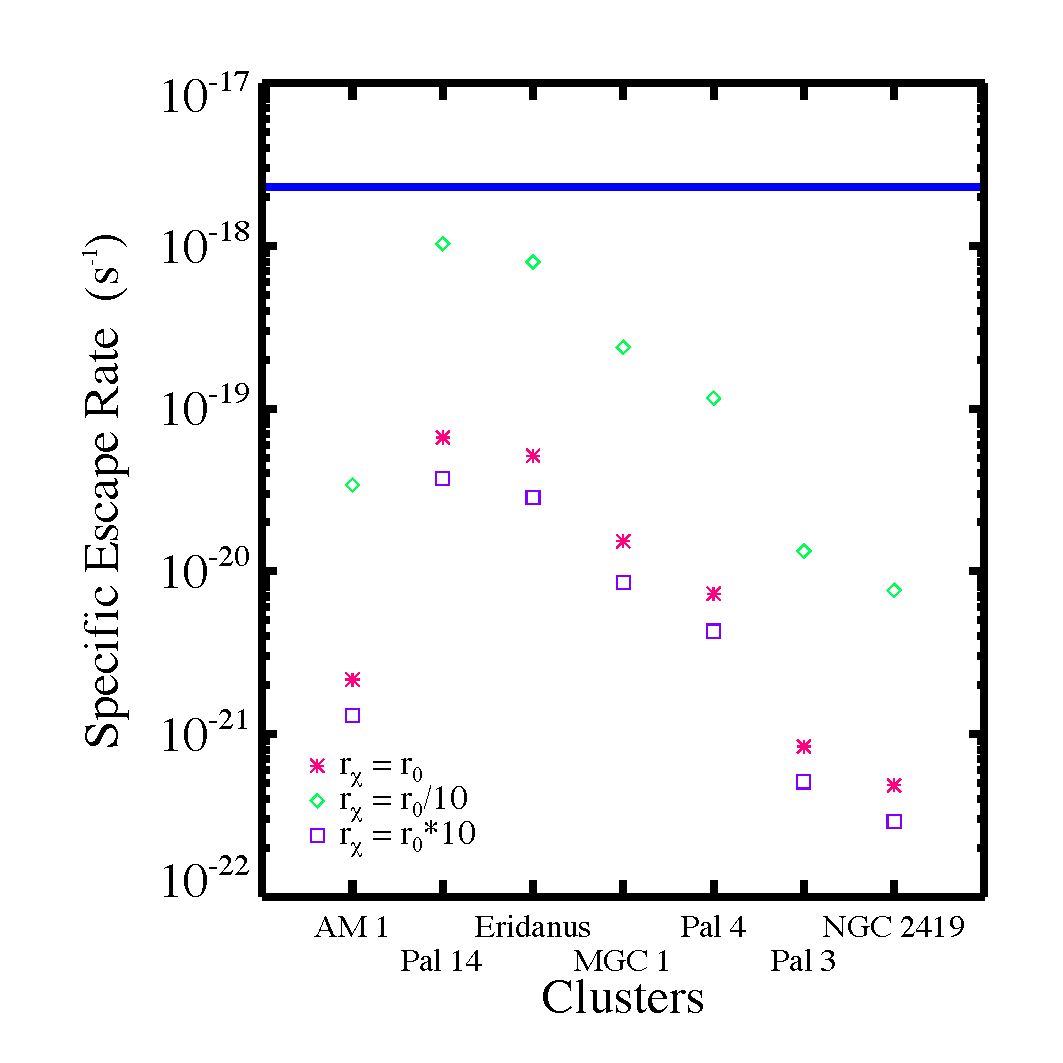
\includegraphics[width=12cm, height=12cm]{var_rad_iso}
\caption{Caption}  
\label{var_rad_iso}
\end{figure}
%
%

%%%%%%%%%%%%%%%%%%%%%%%%%%%%%%%%%%%%%%%%%%%%%%%%%%%
\section{Conclusions}
\label{section:conclusions}


%%%%%%%%%%%%%%%%%%%%%%%%%%%%%%%%%%%%%%%%%%%%%%%%%%%
\acknowledgments

%%%%%%%%%%%%%%%%%%%%%%
\bibliography{Biblio}
%%%%%%%%%%%%%%%%%%%%%%

\end{document}



